 \documentclass{article}

\usepackage{fancyhdr}
\usepackage{extramarks}
\usepackage{amsmath}
\usepackage{amsthm}
\usepackage{amsfonts}
\usepackage{amssymb}
\usepackage{xparse}
\usepackage{tikz}
\usepackage{graphicx}
\usepackage[plain]{algorithm}
\usepackage{algpseudocode}
\usepackage{listings}
\usepackage{hyperref}
\usepackage[per-mode = fraction]{siunitx}
\usepackage{calc}

\usetikzlibrary{automata,positioning}

\hypersetup{
    colorlinks=true,
    linkcolor=blue,
    filecolor=magenta,
    urlcolor=blue,
    }

\urlstyle{same}

%
% Basic Document Settings
%

\topmargin=-0.45in
\evensidemargin=0in
\oddsidemargin=0in
\textwidth=6.5in
\textheight=9.0in
\headsep=0.25in

\linespread{1.1}

\pagestyle{fancy}
\lhead{\hmwkAuthorName}
\chead{\hmwkClass\ (\hmwkClassInstructor,\ \hmwkClassTime): \hmwkTitle}
\rhead{\firstxmark}
\lfoot{\lastxmark}
\cfoot{\thepage}

\renewcommand\headrulewidth{0.4pt}
\renewcommand\footrulewidth{0.4pt}

\setlength\parindent{0pt}
\allowdisplaybreaks
%
% Title Page
%

\title{
	\vspace{2in}
	\textmd{\textbf{\hmwkClass:\ \hmwkTitle}}\\
	\normalsize\vspace{0.1in}\small{Due\ on\ \hmwkDueDate\ at \hmwkDueTime}\\
	\vspace{0.1in}\large{\textit{\hmwkClassInstructor,\ \hmwkClassTime}}
	\vspace{3in}
}
\author{\textbf{\hmwkAuthorName}}
\date{\hmwkCompletionDate}

%
% Create Problem Sections
%

\newcommand{\enterProblemHeader}[1]{
	\nobreak\extramarks{}{Problem #1 continued on next page\ldots}\nobreak{}
	\nobreak\extramarks{Problem #1 (continued)}{Problem #1 continued on next page\ldots}\nobreak{}
}

\newcommand{\exitProblemHeader}[1]{
	\nobreak\extramarks{Problem #1 (continued)}{Problem #1 continued on next page\ldots}\nobreak{}
	\nobreak\extramarks{Problem #1}{}\nobreak{}
}

%
% Homework Problem Environment
%
\NewDocumentEnvironment{hwkProblem}{m m s}{
	\section*{Problem #1: #2}
	\enterProblemHeader{#1}
	\setcounter{partCounter}{1}
}{
	\exitProblemHeader{#1}
	\IfBooleanF{#3} % if star, no new page
		{\newpage}
}

% Alias for the Solution section header
\newcommand{\hwkSol}{\vspace{\baselineskip / 2}\textbf{\Large Solution}\vspace{\baselineskip / 2}}

% Alias for the Solution Part subsection header
\newcounter{partCounter}
\newcommand{\hwkPart}{
	\vspace{\baselineskip / 2}
	\textbf{\large Part \Alph{partCounter}}
	\vspace{\baselineskip / 2}
	\stepcounter{partCounter}
}

%
% Various Helper Commands
%

% Such That
\newcommand{\st}{\text{s.t.}}

% Useful for algorithms
\newcommand{\alg}[1]{\textsc{\bfseries \footnotesize #1}}

% For derivatives
\newcommand{\deriv}[1]{\frac{\mathrm{d}}{\mathrm{d}x} (#1)}

% For partial derivatives
\newcommand{\pderiv}[2]{\frac{\partial}{\partial #1} (#2)}

% Integral dx
\newcommand{\dx}{\mathrm{d}x}
\newcommand{\dy}{\mathrm{d}y}

% Probability commands: Expectation, Variance, Covariance, Bias
\newcommand{\e}[1]{\mathrm{e}#1}
\newcommand{\E}{\mathrm{E}}
\newcommand{\Var}{\mathrm{Var}}
\newcommand{\Cov}{\mathrm{Cov}}
\newcommand{\Bias}{\mathrm{Bias}}

% Defining Units that are not in the SI base
\DeclareSIUnit\bar{bar}
\DeclareSIUnit\ft{ft}
\DeclareSIUnit\dollar{\$}
\DeclareSIUnit\cent{\text{\textcent}}
\DeclareSIUnit\c{\degreeCelsius}

% Code Listing config
\usepackage{xcolor}
\definecolor{codegreen}{rgb}{0,0.6,0}
\definecolor{codegray}{rgb}{0.5,0.5,0.5}
\definecolor{codepurple}{rgb}{0.58,0,0.82}
\definecolor{backcolour}{rgb}{0.95,0.95,0.92}
\lstdefinestyle{overleaf}{
	% backgroundcolor=\color{backcolour},
	commentstyle=\color{codegreen},
	keywordstyle=\color{magenta},
	numberstyle=\tiny\color{codegray},
	stringstyle=\color{codepurple},
	basicstyle=\ttfamily\footnotesize,
	breakatwhitespace=false,
	breaklines=true,
	captionpos=b,
	keepspaces=true,
	numbers=left,
	numbersep=5pt,
	showspaces=false,
	showstringspaces=false,
	showtabs=false,
	tabsize=4
}

\usepackage[latte]{catppuccinpalette}
\lstdefinestyle{catppuccin}{
	breaklines=true,
	keepspaces=true,
	numbers=left,
	numbersep=5pt,
	showspaces=false,
	showstringspaces=false,
	breakatwhitespace=true,
	tabsize=4,
	stringstyle = {\color{CtpGreen}},
	commentstyle={\color{CtpOverlay1}},
	basicstyle = {\small\color{CtpText}\ttfamily},
	keywordstyle = {\color{CtpMauve}},
	keywordstyle = [2]{\color{CtpBlue}},
	keywordstyle = [3]{\color{CtpYellow}},
	keywordstyle = [4]{\color{CtpLavender}},
	keywordstyle = [5]{\color{CtpPeach}},
	keywordstyle = [6]{\color{CtpTeal}}
}

\lstset{style=catppuccin}


%
% Homework Details
%   - Title
%   - Due date
%   - Class
%   - Section/Time
%   - Instructor
%   - Author
%

\newcommand{\hmwkTitle}{Homework 01}
\newcommand{\hmwkDueDate}{September 06, 2024}
\newcommand{\hmwkDueTime}{01:00 PM}
\newcommand{\hmwkClass}{ENAE 301}
\newcommand{\hmwkClassTime}{Section 0103}
\newcommand{\hmwkClassInstructor}{Dr. Paley}
\newcommand{\hmwkAuthorName}{\textbf{Vai Srivastava}}

\begin{document}

\maketitle

\pagebreak

\begin{homeworkProblem}

	\textbf{1.1:} What are the Cartesian coordinates of point \( P \) in frame \( I \), as shown in the following figure?

	\begin{figure}[ht]
		\begin{center}
			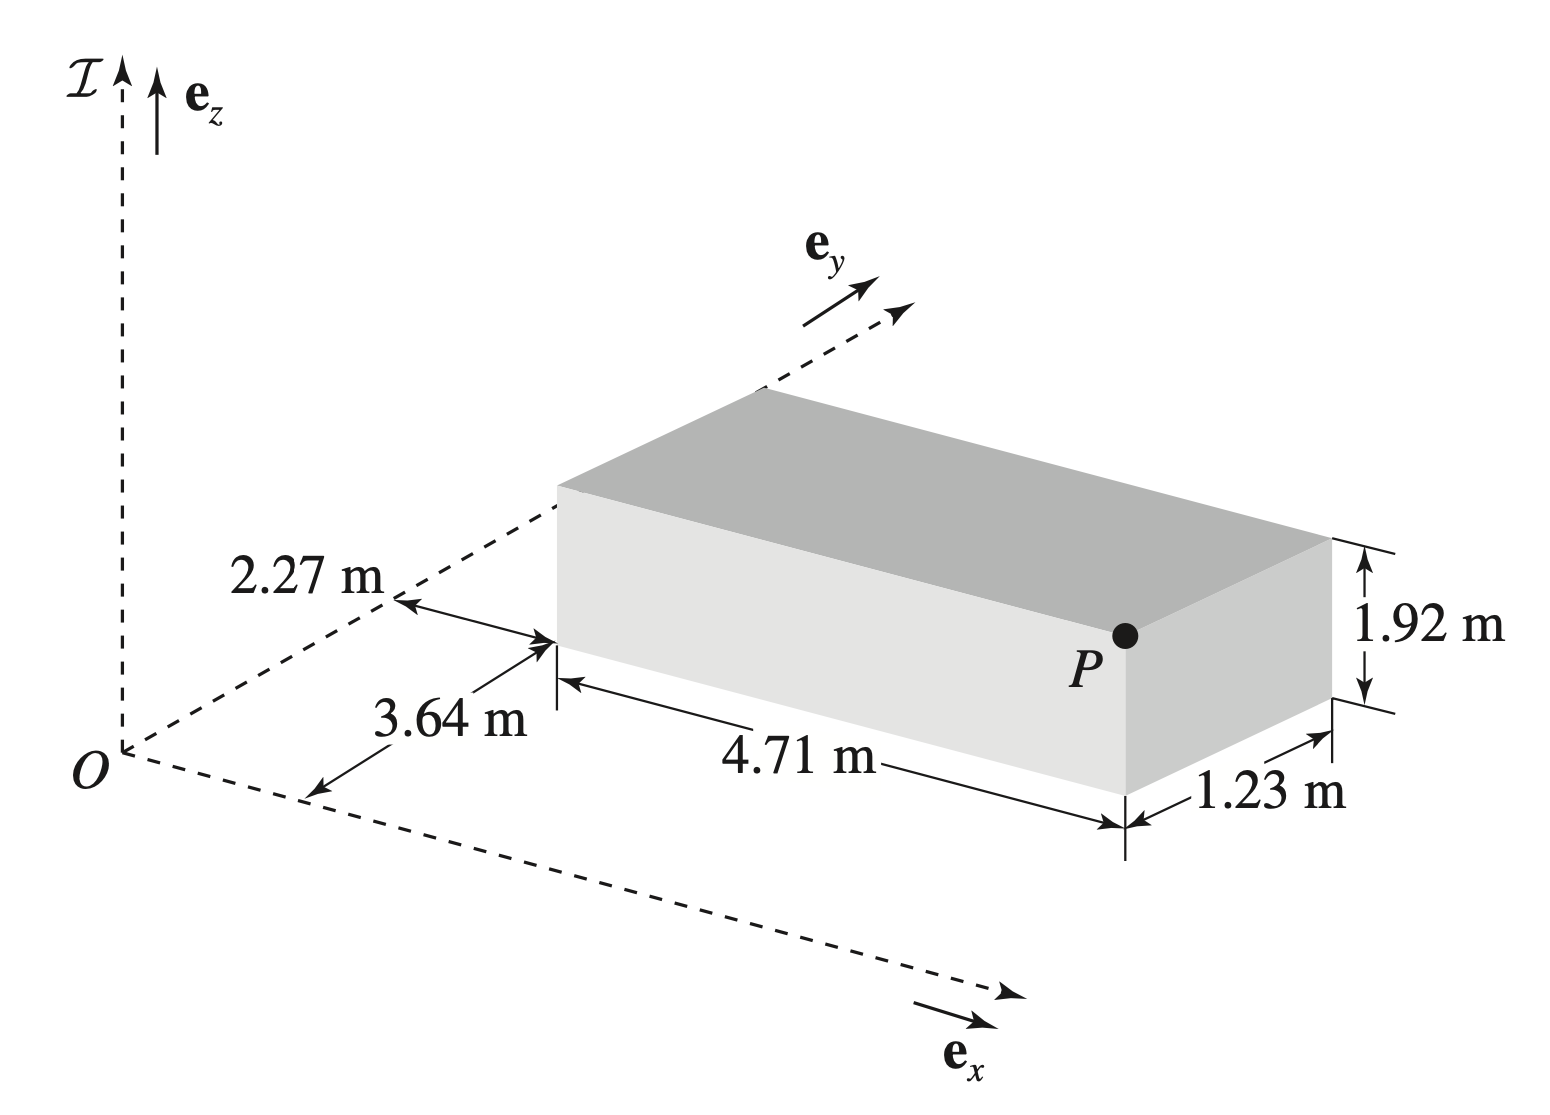
\includegraphics[width=0.65\textwidth]{images/01-1.1.png}
		\end{center}
	\end{figure}

	\solution

	The cartesian coordinates of point \( P \) in frame \( I \) are \( \left(6.98, 3.64, 1.92\right) \) m.

\end{homeworkProblem}

\begin{homeworkProblem}

	\textbf{1.2:} Sketch and label the vectors \( \vec{r}_{\frac{P}{O}} \), \( \vec{r}_{\frac{P}{Q}} \), \( \vec{r}_{\frac{Q}{P}} \) in the following figure:

	\begin{figure}[ht]
		\begin{center}
			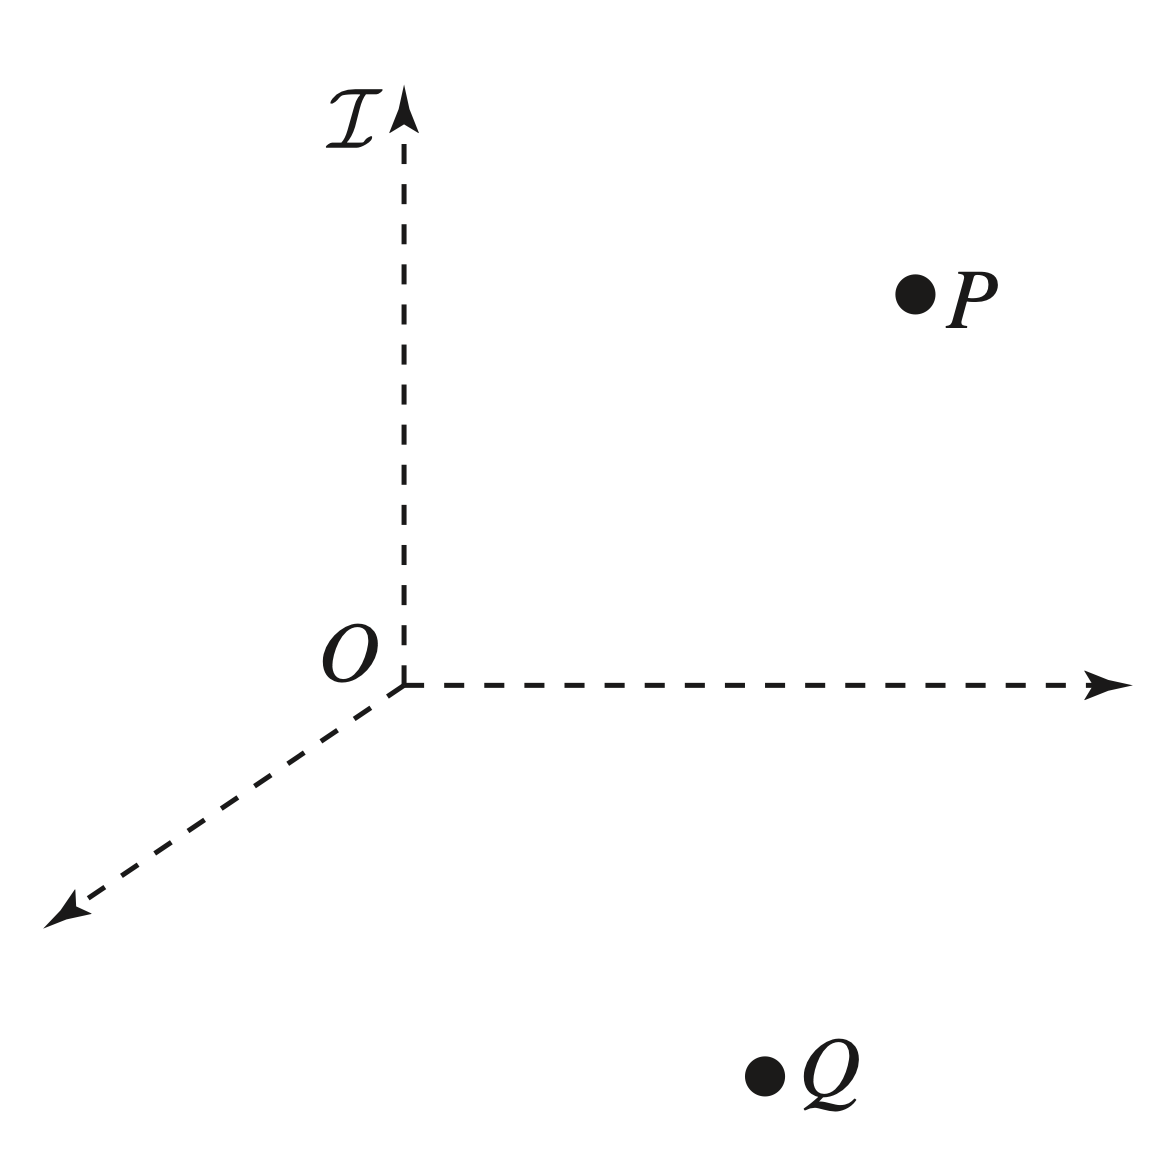
\includegraphics[width=0.45\textwidth]{images/01-1.2.png}
		\end{center}
	\end{figure}

	\solution

	\begin{figure}[ht]
		\begin{center}
			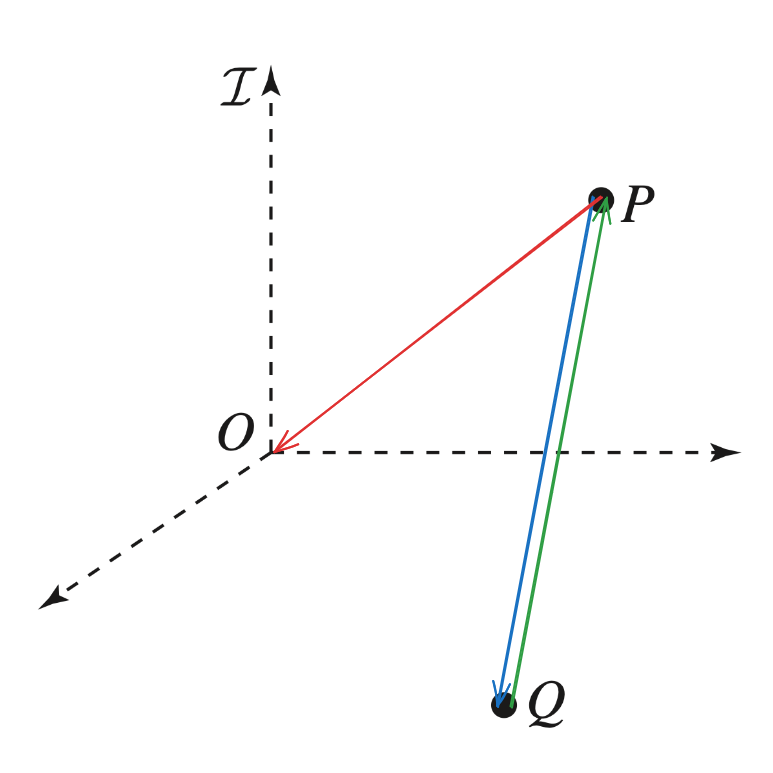
\includegraphics[width=0.45\textwidth]{images/solution 01-1.2.png}
		\end{center}
	\end{figure}

\end{homeworkProblem}

\begin{homeworkProblem}

	\textbf{1.3:} Match each of the following definitions to the appropriate term below:
	\begin{enumerate}
		\item A perspective for observations regarding the motion of a system
		\item A mathematical quantity with both magnitude and direction
		\item Second-order differential equations whose solution is the trajectory of a point
		\item A set of scalars used to locate a point relative to another point
	\end{enumerate}
	\begin{itemize}
		\item Vector
		\item Reference frame
		\item Coordinate system
		\item Equations of motion
	\end{itemize}

	\solution

	\part

	Reference Frame: A perspective for observations regarding the motion of a system.

	\part

	Vector: A mathematical quantity with both magnitude and direction.

	\part

	Equations of motion: Second-order differential equations whose solution is the trajectory of a point.

	\part

	Coordinate system: A set of scalars used to locate a point relative to another point.

\end{homeworkProblem}

\begin{homeworkProblem}

	\textbf{2.3:} Consider the straight-line motion of a particle of mass \( m_{P} \) acted on only by air resistance, \( F_{P} = - b \dot{x}^{2} \). Find analytically an expression for the velocity of the particle as a function of time if it starts with initial velocity \( v_{0} \) at time \( t_{0} \).

	\solution

	\begin{align*}
		m_{P} \frac{d\dot{x}}{dt}                             = F_{P}                                     \\
		m_{P} \frac{d\dot{x}}{dt}                             = -b\dot{x}^{2}                             \\
		\frac{d\dot{x}}{\dot{x}^2}                            = - \frac{b}{m_{P}} dt                      \\
		\left[ - \frac{1}{\dot{x}} \right]^{\dot{x}}_{v_{0}}  = - \frac{b}{m_{P}}\left( t - t_{0} \right) \\
		\dot{x}                                               = \left[ v_{0}^{-1} + \frac{b}{m_{P}} \left( t - t_{0} \right) \right] \qed
		.\end{align*}


\end{homeworkProblem}

\begin{homeworkProblem}

	\textbf{2.6:} Sketch a planar model of a weightlifter's barbell using two point masses and a rigid massless rod. How many degrees of freedom are there in your model?

	\solution

	In my model, there are 3 degrees of freedom.
	\begin{figure}[ht]
		\begin{center}
			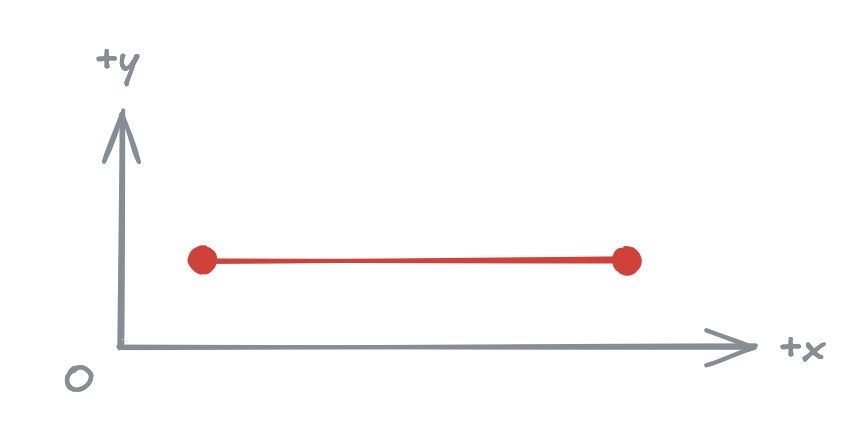
\includegraphics[width=0.45\textwidth]{images/solution 01-2.6.png}
		\end{center}
	\end{figure}

\end{homeworkProblem}

\begin{homeworkProblem}

	\textbf{2.7:} In Example 2.5 we found that the three-link robot arm in Figure 2.6a has three degrees of freedom. We described them by three angles in Figure 2.6b. Suppose, instead, you desired to describe the system by the six Cartesian coordinates for the end of each link, \( \left( x_{1}, y_{1} \right)_{I} \) , \( \left( x_{2}, y_{2} \right)_{I} \), \( \left( x_{3}, y_{3} \right)_{I} \). How many constraint equations would be necessary and what are they?

	\solution

	For this description of the system, we would need two constraint equations:
	\begin{align*}
		r_{a} = \sqrt{\left( x_{1} - x_{2} \right)^2 + \left( y_{1} - y_{2} \right)^2} \\
		r_{b} = \sqrt{\left( x_{2} - x_{3} \right)^2 + \left( y_{2} - y_{3} \right)^2}
		.\end{align*}

\end{homeworkProblem}

\begin{homeworkProblem}

	\textbf{2.12:} Find the equations of motion for a mass m suspended vertically from a spring as shown in the following figure, assuming that the mass is constrained to move only vertically and that it is subject to the force of gravity. Draw a free-body diagram, choose a coordinate system, and use Newton’s second law to find the equation of motion.

	\begin{figure}[ht]
		\begin{center}
			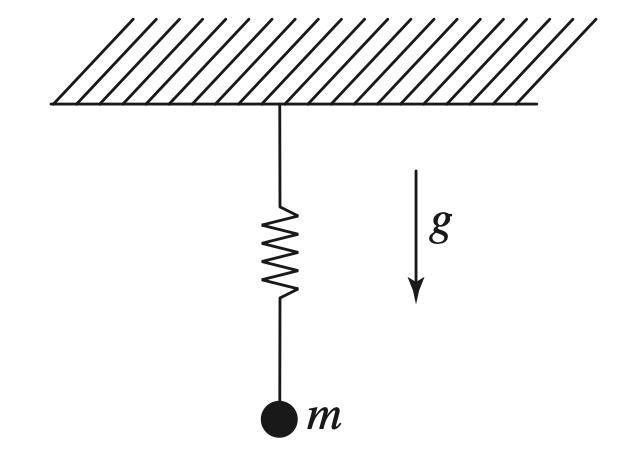
\includegraphics[width=0.45\textwidth]{images/01-2.12.png}
		\end{center}
	\end{figure}

	\solution

	\begin{figure}[ht]
		\begin{center}
			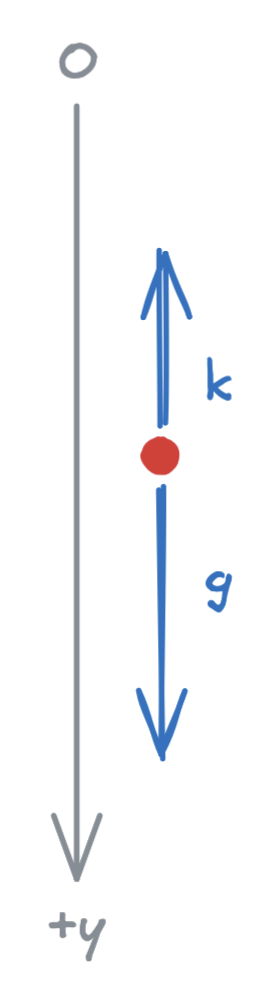
\includegraphics[width=0.15\textwidth]{images/solution 01-2.12.png}
		\end{center}
	\end{figure}

	\[
		\ddot{y} = \frac{g - ky}{m}
		.\]

\end{homeworkProblem}

\begin{homeworkProblem}

	\textbf{2.17:} Consider the equation of motion of a driven simple harmonic oscillator \( \ddot{x} = a - \frac{k}{m} x \), where \( a \) is a constant.
	\begin{enumerate}
		\item Integrate the equation to find the solution analytically.
		\item Solve the equation of motion using \textsc{MATLAB} \lstinline{ODE45}, and plot \( x(t) \) and \( \dot{x}(t) \). Let \( a = 1 \), \( m = 0.5 \), and \( k = 3 \). Be sure to label your axes (with units!) and add a legend to the plot.
	\end{enumerate}

	\solution

	\begin{align*}
		\ddot{x} = a - \frac{k}{m}x                           \\
		d\dot{x} + \frac{k}{m}x = a dt                        \\
		\int \frac{k}{m}x d\dot{x} = \int a dt                \\
		\frac{k}{2m}x^{2} \dot{x} = at + C_{1}                \\
		\frac{k}{2m}x^{2} dx = \left( at + C_{1} \right) dt   \\
		\int \frac{k}{2m}x^{2} dx = \int at + C_{1} dt        \\
		\frac{k}{6m}x^{3} = \frac{a}{2}t^{2} + C_{1}t + C_{2} \\
		x = \sqrt[3]{\left( \frac{a}{2}t^{2} + C_{1}t + C_{2} \right) \frac{6m}{k}} \qed
		.\end{align*}

	Code:
	\begin{lstlisting}[language=MATLAB]
		x0 = [0; 0];
		tspan = [0 10];
		[t, x] = ode45(@harmonic_oscillator, tspan, x0);

		figure;
		subplot(2,1,1);
		plot(t, x(:,1), 'b', 'LineWidth', 2);
		xlabel('Time (s)');
		ylabel('Displacement x(t) (m)');
		title('Displacement vs. Time');
		legend('x(t)');

		subplot(2,1,2);
		plot(t, x(:,2), 'r', 'LineWidth', 2);
		xlabel('Time (s)');
		ylabel('Velocity \dot{x}(t) (m/s)');
		title('Velocity vs. Time');
		legend('\dot{x}(t)');

		grid on;

		function dxdt = harmonic_oscillator(t, x)
		    a = 1;
		    m = 0.5;
		    k = 3;
		    dxdt = zeros(2,1);
		    dxdt(1) = x(2);
		    dxdt(2) = a - (k/m)*x(1);
		end
	\end{lstlisting}

	Plot:
	\begin{figure}[ht]
		\begin{center}
			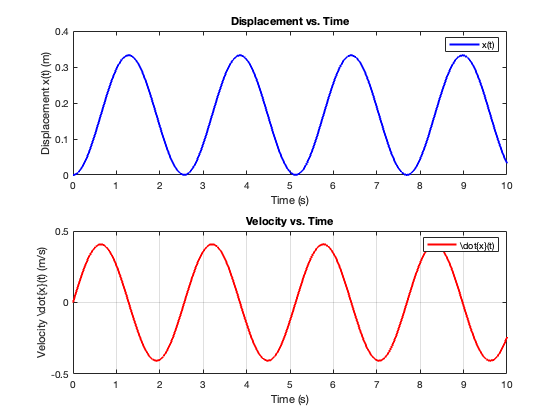
\includegraphics[width=0.85\textwidth]{images/matlab 01-2.17.png}
		\end{center}
	\end{figure}

\end{homeworkProblem}

\end{document}
